%!TEX root = ../AutoML-fuer-Segmentierung.tex
\chapter{NAS-Unet}
\label{ch:nasunet}


% Einträge in die ToDo-Liste setzen (für Änderungen muss 2 mal übersetzt werden, wie bei TOC auch)

\section{Funktionsweise / Theorie}

NAS-Unet ist einer der ersten Versuche NAS auf medizinische Bildsegmentierung anzuwenden. Die folgenden Ausführungen beruhen auf dem Paper \cite{nasunetPaper} von Yu Weng et al.

Es sollten MRT-, CT- und Ultraschallbilder segmentiert werden. Die Architektur von NAS-Unet wurde auf Pascal VOC2012 \cite{PascalVOCDatensatz} gesucht und diese dann auf den unterschiedlichen medizinischen Datensätzen trainiert. Als medizinische Datensätze werden für die MRT-Bilder der Promise12 Datensatz \cite{Promise12Datensatz}, für die CT-Bilder der Chaos Datensatz \cite{ChaosDatensatz} und für die Ultraschallbilder der NERVE Datensatz \cite{NerveDatensatz} verwendet. 

Das vorrangige Ziel von NAS-Unet ist das automatische Finden einer geeigneten Zwei-Zell Architektur. Dabei wird parallel nach der Upsampling und nach der Downsampling Schicht gesucht, die beiden Schichten werden gleichzeitig upgedated. Dabei wird also immer eine Upsampling Zelle gleichzeitig mit der ihr gegenüberliegenden Downsampling Zelle aktualisiert. Die Architektur von NAS-Unet ist streng symmetrisch und es gibt keine zusätzliche Convolutionschicht in der Mitte (siehe Abbildung \ref{pic:nasUnet_ArchitekturGesamt}). 

\begin{figure}[H]
	
	\centering
	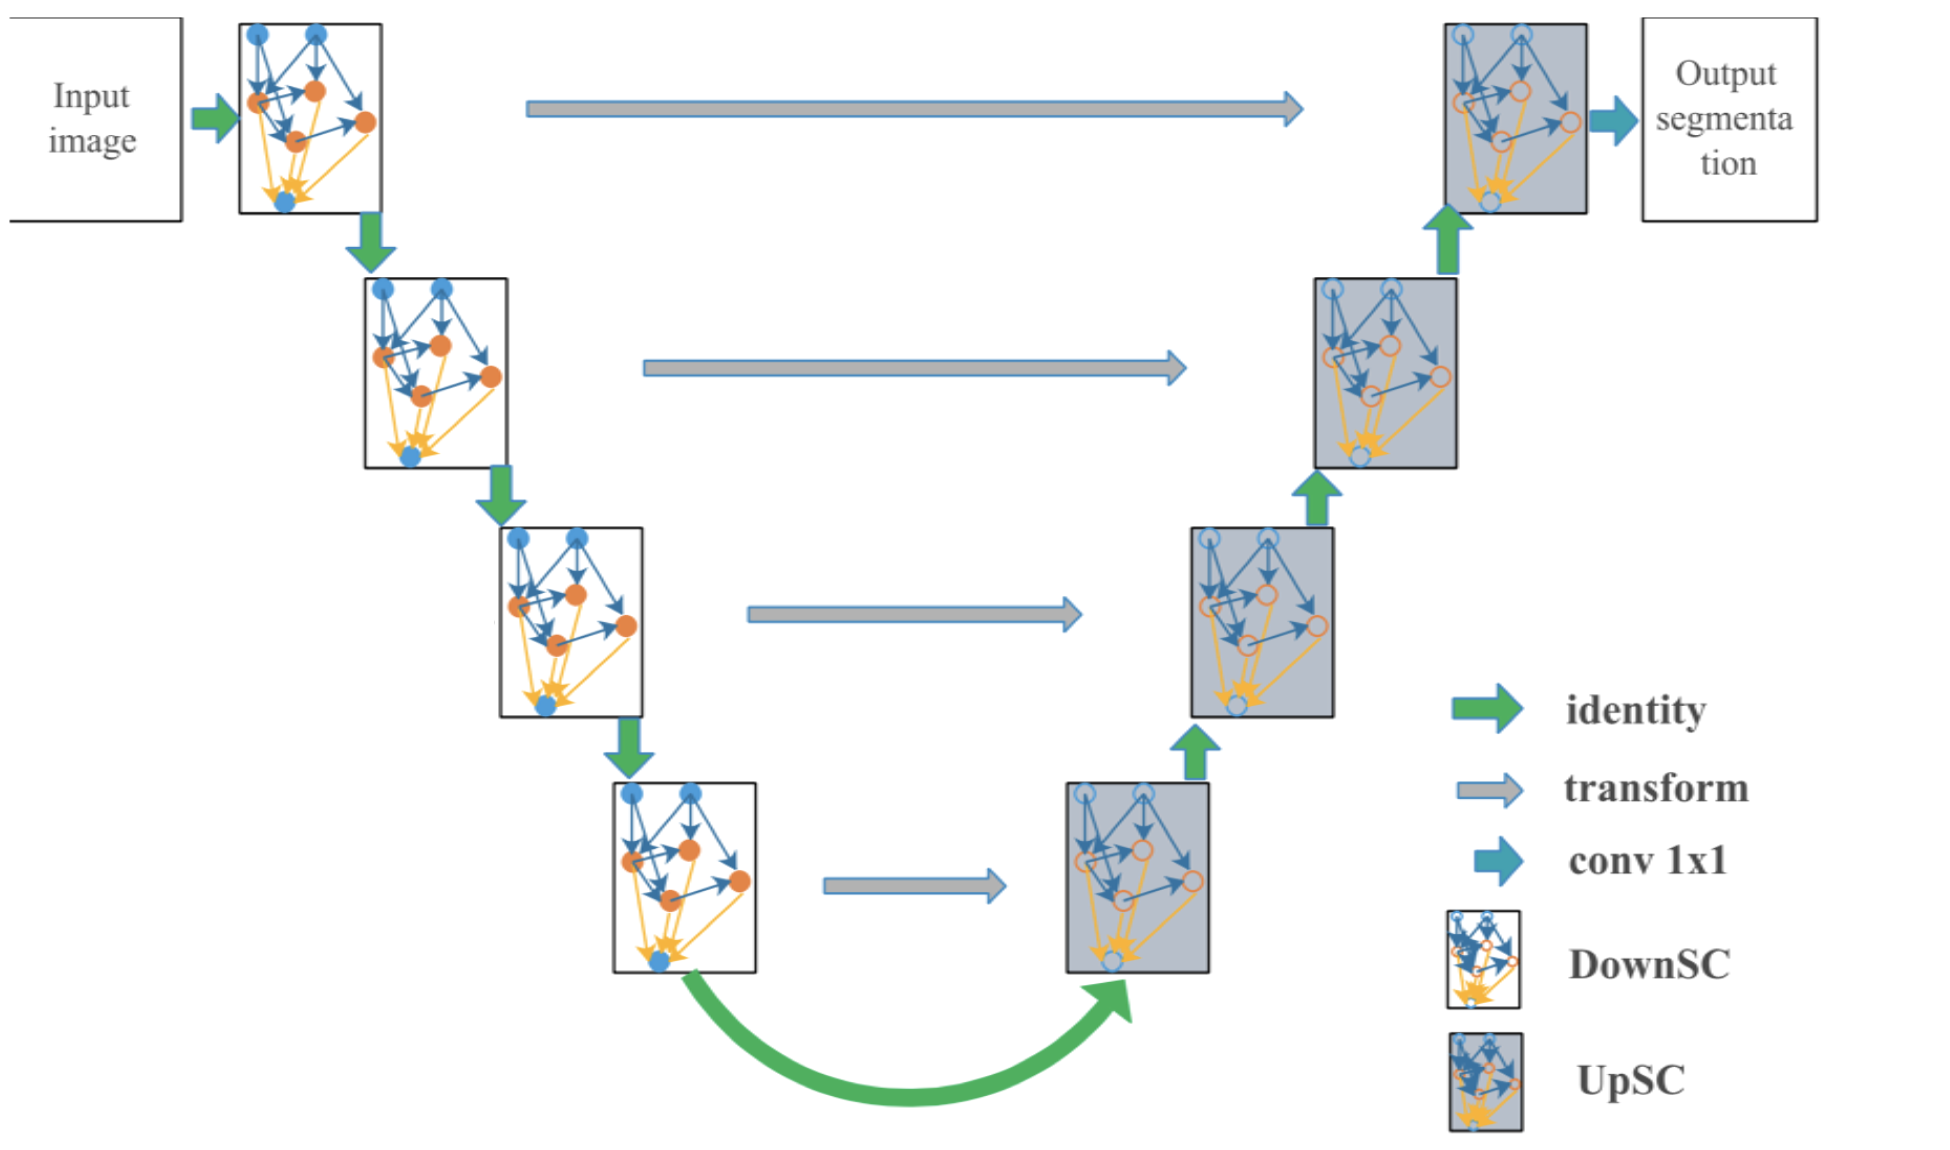
\includegraphics[scale=0.25]{Pictures/nasUnet/Bild1.png}
	\caption{Zellbasierte Netzarchitektur von NAS-Unet \cite{nasunetPaper} }
	\label{pic:nasUnet_ArchitekturGesamt}
\end{figure}

Der Suchraum, in dem die Architektur gesucht werden soll, enthält die möglichen Architekturen, die prinzipiell verwendet werden können, sowie eine Auswahl von primitiven Operationen. Die möglichen Architekturen sind populäre Unet-Architekturen, von denen nur die mittlere Convolutionschicht entfernt wurde. 
NAS-Unet verwendet einen zell-basierten Architektursuchraum. Die zell-basierte Architektur (siehe Abbildung \ref{pic:nasUnet_ArchitekturGesamt}) soll die Generierungsmethode beschränken und so das Problem lösen, dass der Suchraum zu groß wird. Nachdem die beste Zellarchitektur (siehe Abbildung \ref{pic:nasUnet_Zellarchitektur}) gefunden wurde, wird sie im ganzen Netzwerk genutzt und im Rückrad des Netzes gestapelt. Dabei sind nicht nur die Convolutionschichten in die Zellen verlegt, sondern auch alle Up- und Downsampling Operationen. Die Inputknoten einer Schicht sind definiert als die Outputknoten der vorherigen zwei Schichten (siehe Abbildung \ref{pic:nasUnet_Zellarchitektur}). 
Bei der Auswahl der primitiven Operatoren wurde zum einen darauf geachtet Redundanz zu vermeiden und zum anderen darauf, möglichst wenige Parameter zu haben, um möglichst wenig Memory zu verbrauchen. 

\begin{figure}[H]
	
	\centering
	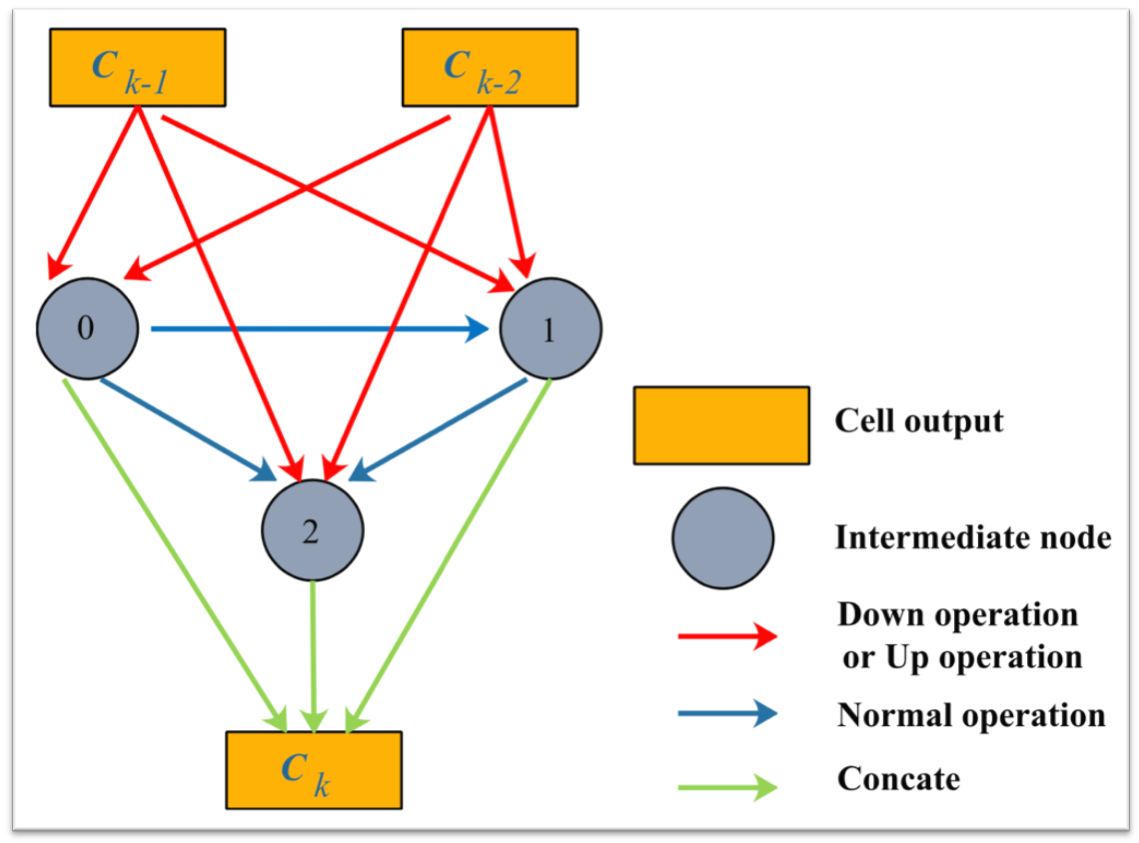
\includegraphics[scale=0.30]{Pictures/nasUnet/Bild2.png}
	\caption{Zellarchitektur von NAS-Unet \cite{nasunetPaper} }
	\label{pic:nasUnet_Zellarchitektur}
\end{figure}

Die Suchstrategie teilt sich in mehrere Schritte auf. Zunächst wird ein überparametrisiertes Netzwerk erstellt (Siehe Abbildung \ref{pic:nasUnet_Zellarchitektur_überparametrisiert}).

\begin{figure}[H]
	
	\centering
	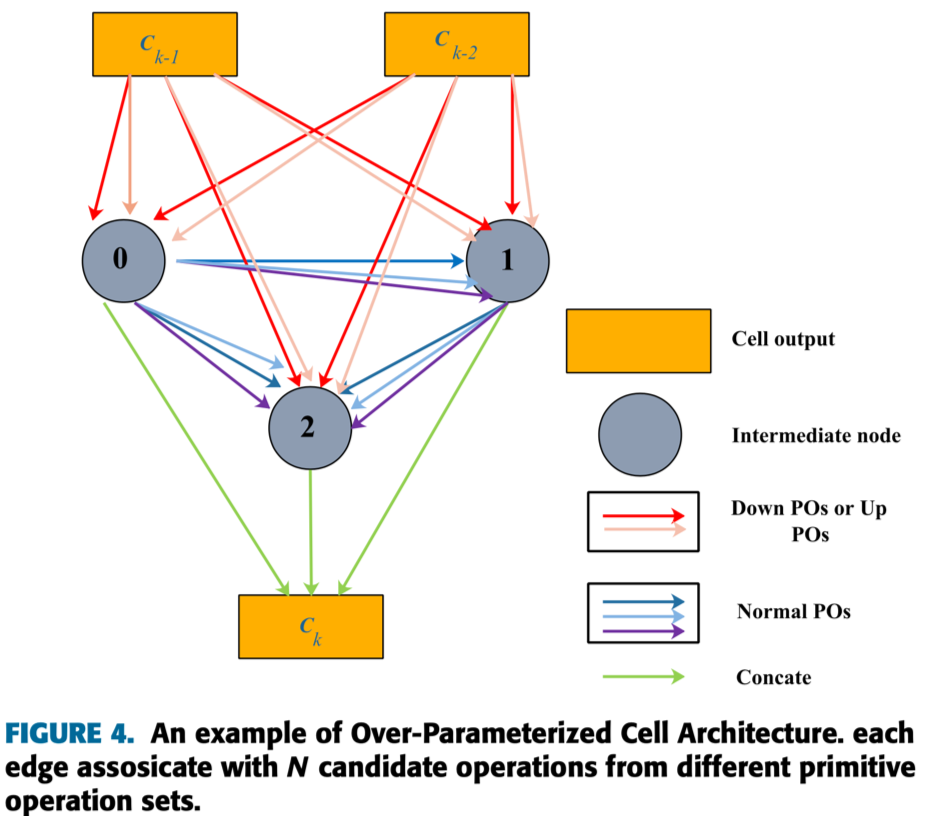
\includegraphics[scale=0.41]{Pictures/nasUnet/Bild3.png}
	\caption{überparametrisierte Zellarchitektur von NAS-Unet \cite{nasunetPaper} }
	\label{pic:nasUnet_Zellarchitektur_überparametrisiert}
\end{figure}


In diesem überparametrisierten Netzwerk lässt sich der Output einer Kante aus der Kombinationen der unterschiedlichen primitiven Operatoren folgendermaßen als Formel darstellen: $$MixO(x)=\sum\limits_{i=1}^{N}w\textsubscript{i}o\textsubscript{i}(x)$$
Dabei ist o(x) die Primitive Operation, w ist das zu der Operation gehörende Gewicht und N ist die Anzahl an primitieven Operationen. 

Um die Parameter zu aktualisieren, wird eine effizienter Parameter-Update Strategie verwendet, damit GPU-Memory gespart wird. Da die Output-Feature-Maps nur berechnet werden können, wenn alle Operationen gleichzeitig im GPU-Memory sind, wird das N-fache an GPU-Memory benötigt, als wenn man ein kompaktes Modell trainieren würde. Daher wird hier ein binärer Ansatz verwendet, das heißt anstatt bei jedem Schritt alle Architekturparameter mit dem Gradientenabstiegsverfahren zu aktualisieren, wird immer nur ein Parameter aktualisiert (siehe Abbildung \ref{pic:nasUnet_binäreSuchstrategie}). Dadurch werden aber mehr Iterationen des Updatens benötigt.

\begin{figure}[H]
	
	\centering
	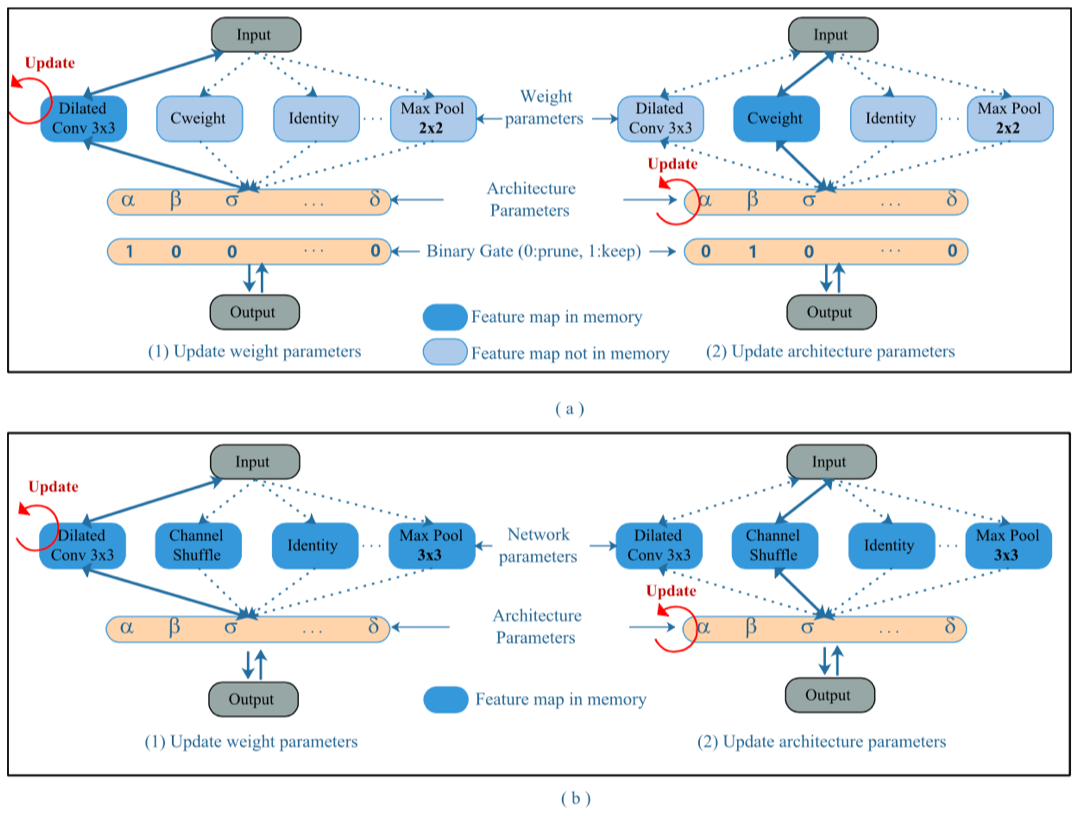
\includegraphics[scale=0.7]{Pictures/nasUnet/Bild4.png}
	\caption{Vergleich der binären Suchstrategie von NAS-Unet mit dem gleichzeitigen Updaten aller Parameter \cite{nasunetPaper} }
	\label{pic:nasUnet_binäreSuchstrategie}
\end{figure}

Zu den Implemetierungsdetails gehört, dass es immer jeweils 4 Up- und Downsampling Zellen gibt. Die Bilder werden zufällig zur einen Hälfte in Trainingsbilder und zur anderen Hälfte in Testbilder eingeteilt. 
Das Paper konzentriert sich vorrangig darauf einen effizienten Suchraum zu konstruieren. Die Suchstrategie ist für die Autoren weniger wichtig, da laut ihrer Aussage (Paper, II. B. \cite{nasunetPaper} und Page 44253, Satz2, \cite{nasunetPaper}) jede differentielle Suchstrategie auf dem Suchraum funtionieren würde. In diesem konkreten Fall wird die DARTS-Update Strategie verwendet. 

\section{Unsere Arbeit / Praxis}

Bei der praktischen Arbeit mit NAS-Unet sind wir auf verschiedene Schwierigkeiten und Hindernisse gestoßen. Diese belaufen sich vorranging auf die Problematik, dass es keine Anleitung oder Einführung für Nas-Unet gibt und auch nahezu keine Dokumentation vorliegt. 
Zunächst einmal haben wir versucht NAS-Unet auf verschiedenen Datensätzen zum Laufen zu bekommen. Dies waren der Datensatz Pascal VOC, der Chaos Datensatz und der Promise Datensatz, welche alle auch im Paper verwendet werden. Bereits hier hatten wie einige Schwierigkeiten, die wir zum Teil auch nicht überwinden konnten. 

Als erstes haben wir durch Fehlermeldungen und Suchen im Code herausgefunden, dass NAS-Unet den Datensatz in einem ganz bestimmten Ordner an einem ganz bestimmten Pfad erwartet. Da wir den Pfad auf Palma nicht einrichten konnten, da dieser schon im Wurzelverzeichnis beginnt, mussten wir die Stelle im Code entsprechend anpassen. Die Tatsache, dass der Code fast gar nicht kommentiert wurde, hat uns die Suche und Anpassung erheblich erschwert. Auch die Ordnernamen und die Struktur des Datensatzes mussten angepasst werden. Auch hierzu gab es keinerlei Hinweise oder Dokumentation. 

Auf dem Chaos Datensatz, welcher auch im Paper verwendet wird, hatten wir das Problem, dass das Framework im Datensatz nach Bildern sucht, die in keiner öffentlich verfügbaren Version des Datensatzes \cite{ChaosDatensatz} existieren. Wie das NAS-Unet auf diese Bilder kommt oder wie man verhindert, dass es nach diesen sucht, ist uns unklar geblieben. 

Während wir den Promise Datensatz nicht öffentlich zugänglich finden konnten, ließ sich das Framework auf dem Pascal VOC Datensatz erfolgreich ausführen. 


\section{Ergebnisse}

Erfolgreich zum Laufen bringen konnten wir das Netz lediglich auf dem Datensatz Pascal VOC2012. Unsere erzielten Ergebnisse waren jedoch leider sehr schlecht. Unsere mIoU auf dem Pascal Datensatz auf den Testbildern war <0.05 (siehe Abbildung \ref{pic:nasUnet_Ergebnisse}). 

\begin{figure}[H]
	
	\centering
	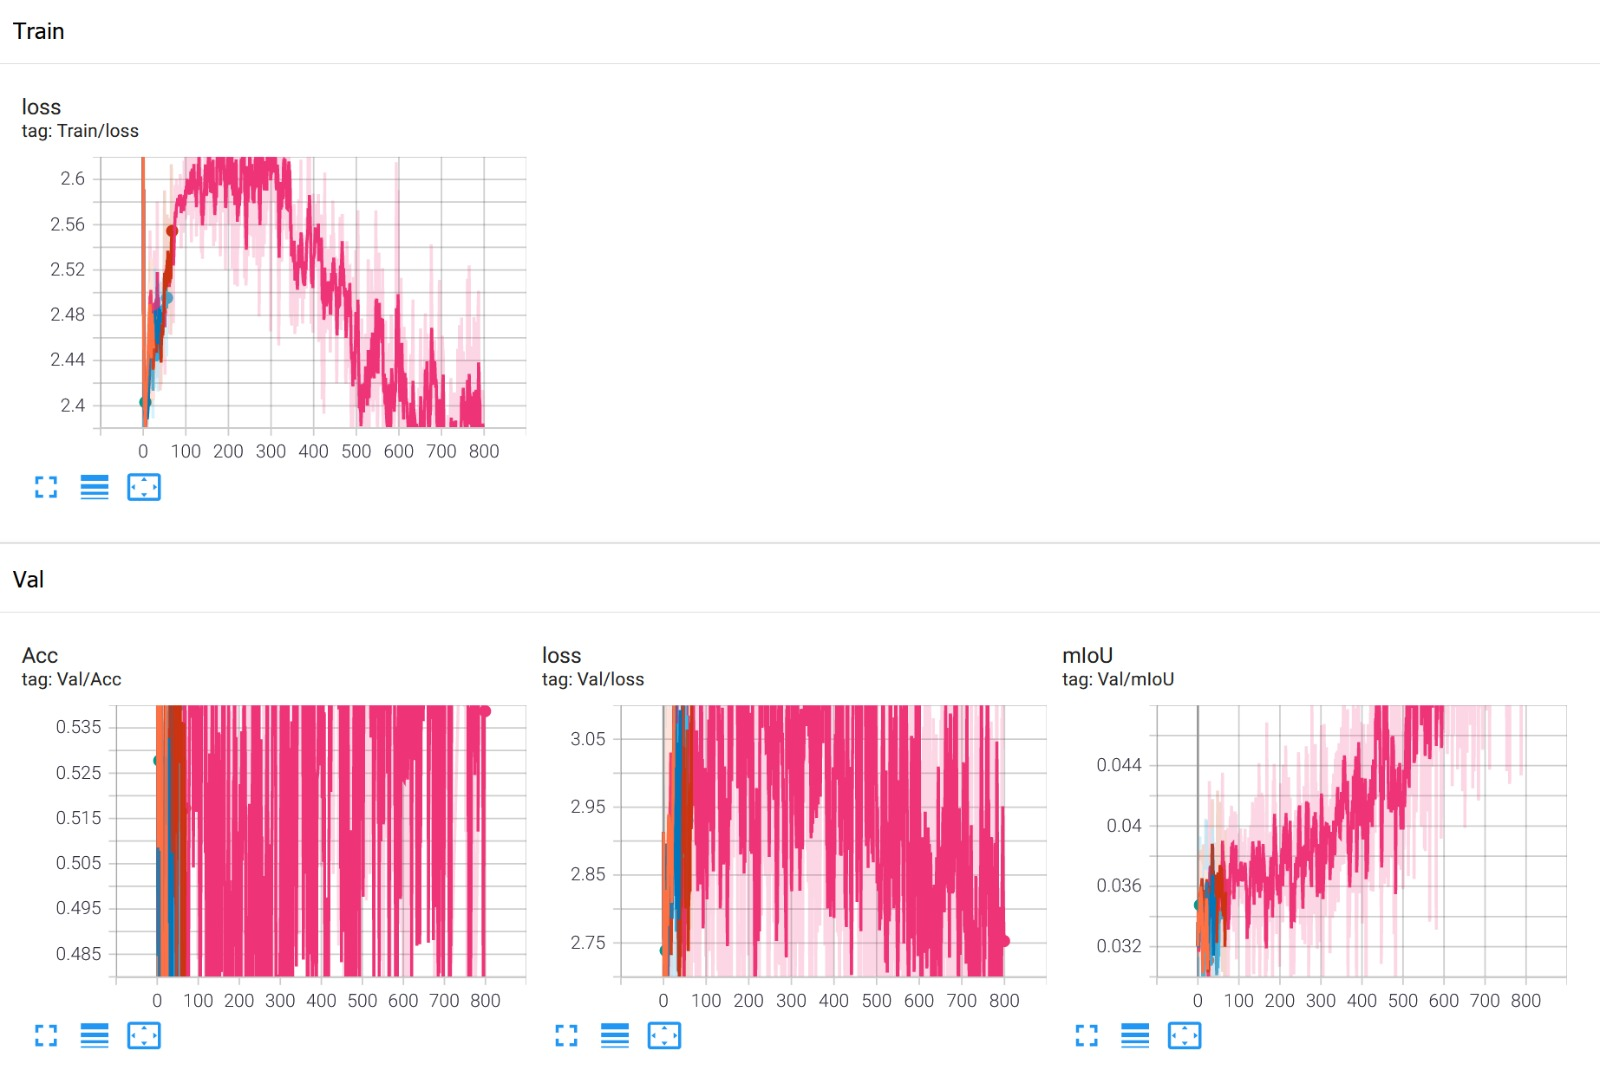
\includegraphics[scale=0.25]{Pictures/nasUnet/Bild5.png}
	\caption{überparametrisierte Zellarchitektur von NAS-Unet \cite{nasunetPaper} }
	\label{pic:nasUnet_Ergebnisse}
\end{figure}

Wie man sieht, ist der Graphenverlauf sehr schwankend und ergibt nur stark gesmoothed eine sichtbare Tendenz. Die Werte sind schlecht bis sehr schlecht, und verbessern sich auch nur sehr langsam.

Auf dem Chaos-Datensatz haben wir NAS-Unet nicht zum Laufen bekommen, da NAS-Unet nach einem Bild sucht, welches in keiner der öffentlichen Versionen des Datensatzes (\cite{ChaosDatensatz} unter Download) existiert. Da es uns nicht gelungen ist, dieses Problem zu lösen, haben wir das Framework leider nicht auf dem Chaos-Datensatz zum Laufen bekommen und können daher auch keine Ergebnisse vorstellen. Uns ist auch nach langer Fehlersuche nicht klar geworden, warum das Framework überhaupt nach einem Bild sucht, welches es eigentlich nie eingegeben bekommen hat. 

Da wir den Promise Datensatz nicht öffentlich finden konnten, können wir hier leider auch über keine Ergebnisse berichten.


\section{Fazit}

Durch die fehlende Dokumentation des Codes und die fehlende Anleitung zur Nutzung des Frameworks ist es extrem schwierig und zeitaufwändig das Framework zu nutzen. Es war uns leider auch nicht möglich, den Code vollständig nachzuvollziehen. Wir konnten daher leider nicht nachvollziehen, was genau gemacht wurde. Auch im Internet, zum Beispiel auf Github, konnten wir leider niemanden finden, der den Code nachvollziehen konnte. Man findet auch hier leider nur viele Fragen. Ein Beispiel ist dieser Versuch den Code nachzuvollziehen ()siehe Abbildung \ref{pic:nasUnet_FrauenhoferScreenshot}) Hier sieht man, dass sich auch die Frage der verschiedenen Metriken auftut. Auch darauf haben wir keine Antwort finden können.

\begin{figure}[H]
	
	\centering
	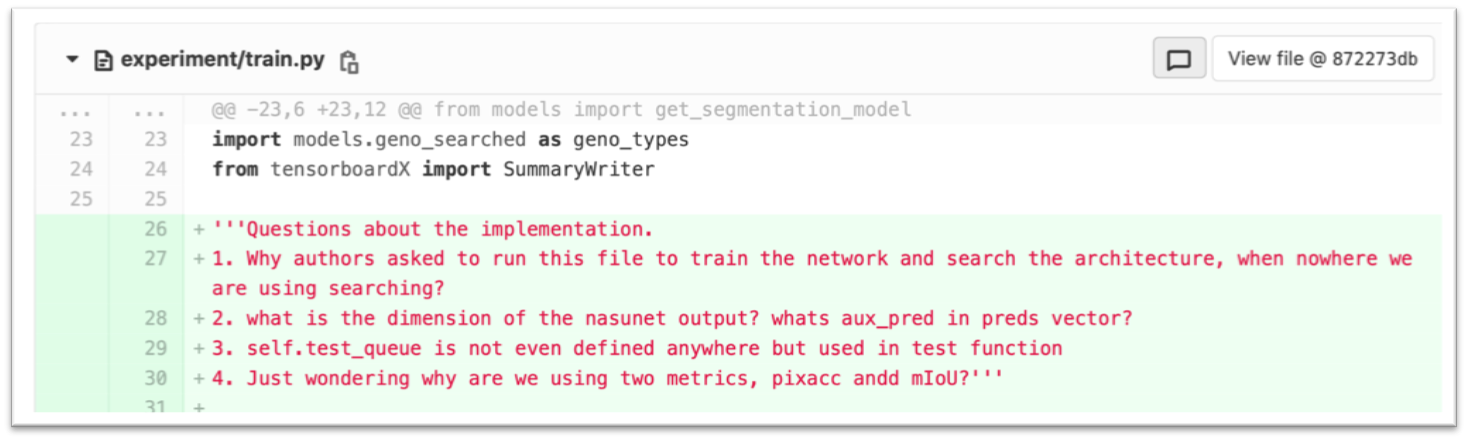
\includegraphics[scale=0.6]{Pictures/nasUnet/Bild6.png}
	\caption{Beispielversuch den Code nachzuvollziehen \cite{Frauenhofer_NasUnet} }
	\label{pic:nasUnet_FrauenhoferScreenshot}
\end{figure}

Ein weiteres Problem ist das Verhalten von NAS-Unet auf dem Chaos Datensatz. Die Frage, warum es nach einem Bild sucht, welches im Datensatz nicht vorkommt, bleibt offen und damit auch die Frage, wie man NAS-Unet auf diesem Datensatz zum Laufen bekommen könnte. Auffällig ist dies vor allem daher, dass NAS-Unet im Paper auch angeblich auf dem Chaos Datensatz angewendet wird. Hier ist wiederum auffällig, dass das Paper zu NAS-Unet am 04.04.2019 veröffentlich wurde, während der Datensatz erst am 11.04.2019 veröffentlich wurde. Möglicherweise hatte die Autoren eine leicht andere Vorversion. Trotzdem erklärt dies nicht, warum das Netz nach mehr Bildern sucht, als ihm eingegeben werden.

Zu den oben genannten Problemen bei der Arbeit mit dem Framework kommt hinzu, dass unsere Ergebnisse auf dem Datensatz Pascal VOC2012 sehr schlecht waren. Besonders auffällig ist dies auf dem Datensatz von Pascal VOC2012, da dieser auch im Paper genutzt wurde und es darauf spezialisiert ist. Leider wurden unserer Recherche nach nie fertig trainierte Modelle von NAS-Unet, welche Ergebnisse wie im Paper angegeben erzielen, veröffentlicht. Daher war es uns leider weder möglich die Ergebnisse zu reproduzieren noch sie nachzuvollziehen.

Im folgenden Github Issue: Issue11 \cite{nasunetGithubIssue11} haben wir herausgefunden, dass man die trainierte Netzstruktur anscheinend händisch in den Code zum Trainieren hineinkopieren muss. Per default verwendet NAS-Unet aber die auf Pascal VOC2012 ausgesuchte Netzstruktur. Daher sollten unsere Ergebnisse auf Pascal VOC 2012 eigentlich davon nicht negativ beeinflusst werden.

Auch beim Durchsuchen der Github Issues auf der zugehörigen Github Seite \cite{nasunetGithub}  sind wir mehrfach darauf gestoßen, dass die Ergebnisse, die im Paper angegeben wurden, nicht reproduziert werden konnten (zum Beispiel Issue 31 \cite{nasunetGithubIssue31}). Da wir auch nicht genau nachvollziehen können, wie diese Ergebnisse entstehen, haben wir uns, auch auf Grund der oben genannten Probleme, dazu entschlossen, nicht länger mit diesem Framework zu arbeiten. Anstelle von NAS-Unet haben wir uns selbstständig ein neues Framework rausgesucht und mit ihm weitergearbeitet (siehe nnU-Net, Kapitel \ref{ch:nnunet}). 



